\documentclass[10pt,twocolumn,letterpaper]{article}

% ============================================================
% TriGate-HDR : Gate-Partitioned Unified Radiance Energy
% CVPR-style submission source
% ============================================================

\usepackage[T1]{fontenc}
\usepackage{times}
\usepackage{amsmath}
\usepackage{amssymb}
\usepackage{amsthm}
\usepackage{graphicx}
\usepackage{booktabs}
\usepackage{float}
\usepackage[breaklinks=true,colorlinks=true,citecolor=blue,linkcolor=blue,urlcolor=blue]{hyperref}
\usepackage[margin=0.75in,columnsep=0.25in]{geometry}
\usepackage{caption}
\usepackage{subcaption}
\usepackage{xcolor}
\usepackage{microtype}
\usepackage{cite}
\usepackage{pifont}

% ---- checkmark / xmark ----
\newcommand{\cmark}{\ding{51}}
\newcommand{\xmark}{\ding{55}}

% ---- self-contained pseudocode (avoids external algorithm* packages) ----
\floatstyle{ruled}
\newfloat{algorithm}{tbp}{loa}
\floatname{algorithm}{Algorithm}
\makeatletter
\newcounter{alg@ln}
\newlength{\alg@ind}
\newenvironment{algorithmic}[1][0]{%
  \setcounter{alg@ln}{0}\setlength{\alg@ind}{0pt}%
  \par\footnotesize\ttfamily
  \begin{list}{}{%
    \setlength{\leftmargin}{1.8em}\setlength{\labelwidth}{1.2em}%
    \setlength{\labelsep}{0.4em}\setlength{\topsep}{2pt}%
    \setlength{\itemsep}{0pt}\setlength{\parsep}{0pt}}%
}{%
  \end{list}\par
}
\newcommand{\alg@item}{\item[\stepcounter{alg@ln}{\scriptsize\arabic{alg@ln}:}]\hspace*{\alg@ind}}
\newcommand{\STATE}{\alg@item}
\newcommand{\FOR}[1]{\alg@item\textbf{for} #1 \textbf{do}\addtolength{\alg@ind}{1.2em}}
\newcommand{\ENDFOR}{\addtolength{\alg@ind}{-1.2em}\alg@item\textbf{end for}}
\newcommand{\IF}[1]{\alg@item\textbf{if} #1 \textbf{then}\addtolength{\alg@ind}{1.2em}}
\newcommand{\ELSE}{\addtolength{\alg@ind}{-1.2em}\alg@item\textbf{else}\addtolength{\alg@ind}{1.2em}}
\newcommand{\ENDIF}{\addtolength{\alg@ind}{-1.2em}\alg@item\textbf{end if}}
\makeatother

% ---- Theorem environments ----
\newtheorem{theorem}{Theorem}
\newtheorem{lemma}{Lemma}
\newtheorem{corollary}{Corollary}
\newtheorem{assumption}{Assumption}
\newtheorem{definition}{Definition}

% ---- Convenience macros ----
\newcommand{\Lrad}{\mathcal{L}_{\mathrm{rad}}}
\newcommand{\Lcold}{\mathcal{L}_{\mathrm{cold}}}
\newcommand{\Lgen}{\mathcal{L}_{\mathrm{gen}}}
\newcommand{\Lbracket}{\mathcal{L}_{\mathrm{bracket}}}
\newcommand{\Lseam}{\mathcal{L}_{\mathrm{seam}}}
\newcommand{\Lgpure}{\mathcal{L}_{\mathrm{GPURE}}}
\newcommand{\zlift}{z^{\mathrm{lift}}}
\newcommand{\zexp}{z^{E}}
\newcommand{\xhdr}{x_{\mathrm{hdr}}}
\newcommand{\xldr}{x_{\mathrm{ldr}}}

\title{\textbf{TriGate-HDR: Gate-Partitioned Unified Radiance Energy for\\
Single-Image HDR Reconstruction via Cold and Generative Diffusion}}

\author{
Anonymous CVPR Submission\\
Paper ID: TBD
}

\date{}

\begin{document}
\twocolumn[
\maketitle
\begin{abstract}
Single-image high dynamic range (HDR) reconstruction is a fundamentally ill-posed inverse problem where a single low dynamic range (LDR) photograph must yield a physically accurate radiance map across regions that are either saturated or severely underexposed. Prior work either addresses this through cascaded pipeline stages trained in isolation or through unified generative frameworks that apply a single prior uniformly across all exposure regimes. We argue that neither approach is optimal: isolated stages cannot jointly minimize a single coherent physical energy, while uniform generative models fail to respect the deterministic radiometric structure of well-exposed pixels.

We introduce TriGate-HDR, a framework built around the Gate-Partitioned Unified Radiance Energy (GPURE) objective that explicitly partitions the LDR input into three regions --- trusted (well-exposed), clipped (saturated), and a seam band between them --- and routes each region through a complementary generative path. The cold diffusion path (Path-C) applies an expansion-only Log-Radiance Cold Forward Process (LR-CFP) grounded in optical radiometry to trusted regions, while the generative diffusion path (Path-G) applies a masked InstructPix2Pix prior to clipped regions. A differentiable TriGateComposer and a seaming WGAN (Path-S) fuse the two paths and resolve boundary artifacts. All three paths are jointly optimized under a single partitioned variational energy $\Lgpure$ that couples them through Exposure-Bracket Consistency (ECC) on seam bands and Radiometric Synapse Operators (RSO) at skip connections.

Our central theoretical contribution is that LR-CFP establishes a provably identifiable expansion field on trusted pixels under mild monotonicity assumptions, yielding a physically motivated cold forward process that is strictly more constrained than generic cold diffusion. RSO replaces conventional convolutional skip-fusion with a camera-response-aware depthwise Jacobian operator that encodes domain-specific radiometric knowledge. On the HDR-Real benchmark, TriGate-HDR attains a $\mu$-law PSNR of $29.06$~dB, SSIM-$\mu$ of $0.941$, and PSNR-PU of $31.20$~dB, matching or surpassing recent one-step diffusion HDR methods on the majority of full-reference fidelity metrics, while providing interpretable, physically grounded radiance partitioning that is absent from prior frameworks.
\end{abstract}
]

% ============================================================
\section{Introduction}
\label{sec:intro}

Recovering a high dynamic range radiance map from a single low dynamic range photograph sits at the intersection of physics-based inversion and generative image synthesis. The difficulty is structural rather than merely statistical. A camera sensor clips all irradiance values above a saturation threshold to the same maximum digital code, permanently destroying the photon statistics for those pixels. In underexposed regions, quantization and noise corrupt the signal. These two failure modes have fundamentally different optimal treatments: saturated regions require synthesis of plausible radiance from scene context, while well-exposed regions admit a near-deterministic inversion of the camera response function (CRF) and tone curve. Most existing methods either apply a single learned prior uniformly across all regions, ignoring this structural dichotomy, or cascade separately trained modules without a coherent joint optimization objective.

Feed-forward convolutional approaches such as FHDR~\cite{fhdr} and SingleHDR~\cite{singlehdr} model HDR reconstruction as a direct regression and enforce no radiometric structure beyond pixel-wise loss. Diffusion-based methods including LEDiff~\cite{lediff} and the very recent ExpoCM~\cite{expocm} bring generative priors that substantially improve perceptual quality in saturated highlights, yet they apply the same stochastic sampling process to well-exposed pixels where the inverse problem is essentially deterministic, introducing unnecessary variance and potentially violating physical consistency.

We identify the core failure mode as a \emph{regime conflation} problem: applying a single generative objective uniformly across exposure regimes conflates a well-conditioned regression problem (trusted pixels) with a genuinely generative one (clipped pixels). Our answer is to explicitly decompose the LDR image into a trust-gated partition and assign each regime its own physically appropriate operator, while coupling all operators under one joint variational energy so that gradients flow coherently.

\subsection{Contributions}

The key contributions of this work are as follows.

\begin{itemize}
\item We introduce the \textbf{Gate-Partitioned Unified Radiance Energy (GPURE)} framework, which, to our knowledge, is the first HDR reconstruction formulation to unify a cold diffusion radiometric path and a masked generative diffusion path under a single differentiable variational objective.
\item We derive the \textbf{Log-Radiance Cold Forward Process (LR-CFP)} and provide a formal identifiability theorem showing that the expansion latent field on trusted pixels is uniquely determined from paired HDR--LDR data under mild monotonicity assumptions, establishing a stronger theoretical foundation than generic cold diffusion.
\item We propose \textbf{Radiometric Synapse Operators (RSO)} as camera-response-informed skip-level fusion modules that replace generic convolutional gates with physically meaningful log-ratio operators, making the skip fusion interpretable in terms of the CRF.
\item We introduce \textbf{Exposure-Bracket Consistency (ECC)} as a seam-band coupling loss that enforces photometric consistency between Path-G and Path-C along clipping boundaries, mitigating seam artifacts without a separate alignment stage.
\item We present a three-phase joint training procedure (warmup, joint, seam) that efficiently bootstraps from independently pretrained cold and generative models.
\end{itemize}

% ============================================================
\section{Related Work}
\label{sec:related}

\subsection{Single-Image HDR Reconstruction}

The problem of reconstructing a high dynamic range image from a single low dynamic range exposure has a long history stretching back to Debevec and Malik's radiometric calibration work~\cite{debevec1997}. Early deep learning approaches, most notably the HDRCNN of Eilertsen et al.~\cite{hdrcnn}, used convolutional encoders to hallucinate luminance content in saturated regions, framing the problem as masked inpainting in log-luminance space. Liu et al.'s SingleHDR~\cite{singlehdr} decomposed the LDR pipeline into three sequential sub-networks --- dequantization, linearization, and hallucination --- and jointly fine-tuned them end-to-end. The FHDR framework of Khan et al.~\cite{fhdr} introduced a feedback recurrent structure that progressively refines coarse-to-fine HDR estimates over multiple iterations. Santos et al.~\cite{santos2020} combined masked feature learning with VGG-based perceptual losses to better recover fine details in saturated highlights. Barua et al.'s ArtHDR-Net~\cite{arthdr} and HistoHDR-Net~\cite{histohdr} emphasized perceptual quality and histogram-based conditioning respectively. While all of these methods achieve competitive pixel-wise metrics, they apply a single feedforward pass uniformly across all exposure regimes and thus treat the deterministic trusted-pixel inversion and the generative saturated-pixel synthesis as instances of the same regression problem.

\subsection{Diffusion-Based HDR Methods}

The recent surge in diffusion models has spurred a new generation of HDR reconstruction methods that leverage powerful generative priors. LEDiff~\cite{lediff} adapts a pretrained latent diffusion model to HDR generation by fusing exposure-bracket latent codes with a fine-tuned VAE decoder that supports linear HDR output. Bracket Diffusion-style approaches~\cite{exposurediffusion} apply DDPM-like consistency across multiple synthetic exposures derived from the single LDR input, providing exposure diversity through re-rendering rather than multi-shot capture. The concurrent ExpoCM~\cite{expocm} is the closest prior work to our framework: it constructs exposure-aware consistency trajectories via a Probability Flow ODE and a soft exposure mask that partitions the LDR image into over-, under-, and well-exposed regions, then applies region-conditioned hallucination within a distillation-free one-step model. Our work differs from ExpoCM in three fundamental ways. Where ExpoCM applies a single generative ODE conditioned on the exposure mask, GPURE routes distinct complementary generators --- a cold radiometric path and a generative diffusion path --- through physically motivated skip operators. ExpoCM uses Gaussian diffusion noise throughout; GPURE's cold path applies deterministic LDR-anchored corruption restricted to the expansion latent component, exploiting the known LDR observation as a structural anchor. Finally, ExpoCM's exposure partitioning is a soft conditioning mechanism for one generator; GPURE's gate partition determines which generator has gradient ownership over which pixel region.

\subsection{Cold Diffusion}

Cold diffusion was introduced by Bansal et al.~\cite{colddiffusion} as a generalization of the diffusion paradigm that replaces Gaussian noise with arbitrary deterministic corruptions --- blurring, snowification, inpainting masks --- and shows that valid generative models can be built on any such forward process. The key insight is that the model's generative behavior does not strongly depend on the specific choice of corruption as long as the reverse process is trained consistently with it. LR-CFP is a new member of this family: the corruption is LDR-clip blending restricted to the expansion latent, operating in log-radiance space. Unlike generic cold diffusion, LR-CFP comes with domain-specific constraints --- monotonicity of the lift map, trust-gate partitioning, and optical calibration --- that together yield the identifiability theorem in Section~\ref{sec:theorem}. Reti-Diff~\cite{retidiff} applies a Retinex-based latent diffusion framework to illumination-degraded image restoration and similarly separates a reflectance prior from an illumination correction objective in latent space. GPURE differs in that it targets radiance expansion (HDR dynamic range recovery) rather than reflectance normalization, and the two paths are complementary generators rather than a single DM with decomposed input.

\subsection{Instruction-Guided Latent Diffusion}

InstructPix2Pix~\cite{instructpix2pix} introduced the paradigm of conditioning a pretrained latent diffusion model on both an input image and a textual editing instruction, enabling general-purpose image editing from paired synthetic training data. In TriGate-HDR's Stage~1 (Path-G), we fine-tune InstructPix2Pix with LoRA~\cite{lora} adapters and a set of TriGate conditioning encoders that inject material, structural, semantic, and mask features into the image latents. This grounds the generative hallucination in spatial structure derived from the LDR input, reducing ungrounded hallucination artifacts in clipped regions.

\subsection{GAN-Based Seam Refinement}

Compositing-based HDR methods that paste independently generated content into a base image face seam artifacts at paste boundaries. While most methods apply simple alpha blending or morphological smoothing, we argue that a learned adversarial refiner with mask-gated attention is necessary to propagate context across the seam band. Our Stage~3 Seaming WGAN draws on the Wasserstein GAN with gradient penalty (WGAN-GP)~\cite{wgangp} framework with a dual-head PatchGAN discriminator~\cite{pix2pix} that separately evaluates global coherence and local seam quality.

% ============================================================
\section{Method}
\label{sec:method}

TriGate-HDR is a three-path HDR reconstruction framework jointly optimized under the GPURE variational energy. The three paths --- Path-C (cold radiometric), Path-G (generative diffusion), and Path-S (seam adversarial) --- each address a structurally distinct regime of the LDR-to-HDR inverse problem, and they are coupled through a differentiable composition operator and a set of physical consistency losses.

\subsection{Problem Formulation}

Let $\xldr \in [0,1]^{3\times H \times W}$ denote the display-referred LDR image captured by a camera with an unknown camera response function $\Phi$ and a clipping threshold $\theta_{\mathrm{clip}}$. The true scene radiance is denoted $L \in \mathbb{R}_{\geq 0}^{3\times H \times W}$, and the HDR image $\xhdr \in [-1,1]^{3\times H \times W}$ is the per-image max-normalized representation of $L$. The LDR is generated as
\begin{equation}
\xldr = \mathrm{clip}\big(\Phi(L / E),\ 0,\ 1\big),
\label{eq:ldr-formation}
\end{equation}
where $E$ is the exposure factor and $\mathrm{clip}$ saturates all values above $\theta_{\mathrm{clip}} \approx 0.98$. The inverse problem is ill-posed in pixels $u$ where $\max_c \xldr(u,c) \geq \theta_{\mathrm{clip}}$ (the clipped region) and near-deterministic elsewhere. We denote the pixel-wise trust gate $g : \mathbb{R}^{H\times W} \rightarrow \{0,1\}$ as
\begin{equation}
g_u = \mathbf{1}\big[\max_c \xldr(u,c) < \theta_{\mathrm{clip}}\big].
\label{eq:gate}
\end{equation}
This binary gate partitions the spatial domain into trusted pixels ($g_u=1$) and clipped pixels ($g_u=0$). The clip mask $m_{\mathrm{clip}} = 1-g$ and the seam mask $m_{\mathrm{seam}}$ are derived from $g$ via morphological dilation and erosion:
\begin{equation}
m_{\mathrm{seam}} = \mathrm{clip}\big(\mathrm{dilate}(m_{\mathrm{clip}}) - \mathrm{erode}(m_{\mathrm{clip}})\big) \,\vee\, m_{\mathrm{clip}}.
\label{eq:seam-mask}
\end{equation}

\subsection{Stage 1 --- Path-G: Masked Generative Diffusion}

Path-G provides a hallucination prior for saturated regions by fine-tuning an InstructPix2Pix~\cite{instructpix2pix} latent diffusion UNet with LoRA adapters and TriGate conditioning encoders. The forward process in Stage~1 is standard Gaussian diffusion:
\begin{equation}
z_t = \sqrt{\bar\alpha_t}\, z_{\mathrm{hdr}} + \sqrt{1-\bar\alpha_t}\,\epsilon, \quad \epsilon \sim \mathcal{N}(0,I).
\label{eq:gaussian-fwd}
\end{equation}
The TriGate conditioning system injects spatial structure from the LDR through four specialized encoders: the Material Encoder $E_m$ extracts texture and material cues; the Structural Encoder $E_s$ extracts geometry and the trust gate $g$; the Semantic Codebook Encoder $E_{\mathrm{sem}}$ produces VAE-style latent codes with KL regularization; and the Mask Encoder $E_{\mathrm{mask}}$ encodes SAM-derived~\cite{sam} semantic regions. The encoded features are fused by the HorizontalTriStreamFusion module via timestep-gated cross-attention:
\begin{align}
\mathrm{Attn}_S &= \mathrm{softmax}\!\left(\frac{Q_M K_S^\top}{\sqrt{C}}\right) V_S, \\
\mathrm{Attn}_Z &= \mathrm{softmax}\!\left(\frac{Q_M K_Z^\top}{\sqrt{C}}\right) V_Z, \\
\mathrm{fused} &= [\gamma_1 \tilde M,\ \gamma_2 \mathrm{Attn}_S,\ \gamma_3 \mathrm{Attn}_Z,\ \gamma_4 \tilde R],
\label{eq:tristream}
\end{align}
where $\gamma_k = \sigma(W_k t_{\mathrm{emb}})$ are learned timestep gates. The fused conditioning is injected into the image latents $z_{\mathrm{img}}$ as a residual with a learnable scalar $\sigma_{\mathrm{res}}$ (initialized to $0.1$). Stage~1 is pretrained using the diffusion loss $\mathcal{L}_{\mathrm{diff}} = \|\hat\epsilon - \epsilon\|_2^2$ and then augmented with perceptual losses W1 (Wasserstein-1 in feature space), SFL (structural fidelity loss), and KL on semantic latents.

\subsection{Stage 2 --- Path-C: Cold Radiometric Expansion}

Path-C is the core radiometric engine of TriGate-HDR. It applies a deterministic cold forward process restricted to the expansion component of the HDR latent, with the LDR serving as a fixed structural anchor. Unlike Path-G, Stage~2 is trained from scratch with a purpose-built MiniHDR-VAE (no pretrained SD/CLIP backbone).

\subsubsection{Log-Radiance Cold Forward Process (LR-CFP)}

The LR-CFP encodes inputs in log-radiance space before VAE compression, providing optical calibration consistent with photometric theory. For an HDR tensor $x \in [-1,1]^3$, the LR-CFP encoding is
\begin{equation}
\ell(x) = \frac{\log\big(1 + k \odot \max(\mathrm{radiance}(x), 0)\big)}{s},
\label{eq:lrcfp}
\end{equation}
where $k \in \mathbb{R}^3$ is a per-channel learnable gain (\texttt{OpticalColdForward.k}) and $s$ is a normalization scale. The MiniHDR-VAE then encodes $\ell(x)$ into the latent space:
\begin{equation}
z_{\mathrm{HDR}} = E(\ell(\xhdr)), \qquad z_{\mathrm{LDR}} = E(\ell(x_{\mathrm{ldr}}^{\mathrm{hdr}})),
\label{eq:vae-encode}
\end{equation}
where $x_{\mathrm{ldr}}^{\mathrm{hdr}} = 2\xldr - 1$ maps the LDR to HDR range. The MonoLift module $\mathcal{M}$ computes a latent anchor:
\begin{equation}
\zlift = \mathcal{M}(z_{\mathrm{LDR}}) = z_{\mathrm{LDR}} + \mathrm{net}(z_{\mathrm{LDR}}),
\label{eq:monolift}
\end{equation}
with a monotonicity penalty enforcing that $\mathcal{M}$ is non-decreasing in latent space. The expansion field is
\begin{equation}
z_0^{E} = z_{\mathrm{HDR}} - \zlift.
\label{eq:expansion-field}
\end{equation}
The cold forward process corrupts only the expansion component:
\begin{equation}
z_t^{E} = (1-\alpha_t)\, z_0^{E}, \qquad z_t = \zlift + z_t^{E}, \qquad \alpha_t = \frac{t}{T-1}.
\label{eq:cold-fwd}
\end{equation}
Note that Gaussian noise is never added: the corruption is a deterministic blend toward zero expansion, with the LDR anchor $\zlift$ held fixed. At $t=T-1$, the expansion has fully collapsed ($z^E=0$) and the state equals the LDR lift --- not a noise-corrupted version. This is the key property that distinguishes LR-CFP from both warm Gaussian diffusion and generic Bansal cold diffusion.

\subsubsection{Identifiability Theorem}
\label{sec:theorem}

The following theorem justifies the expansion-only cold parameterization and distinguishes LR-CFP from the generic cold framework of Bansal et al.~\cite{colddiffusion}.

\begin{assumption}[Monotone Lift]
$\mathcal{M}$ is monotone in latent space, enforced by the monotonicity penalty $\mathcal{L}_{\mathrm{mono}} = \mathbb{E}[\max(0, -\partial \mathcal{M}/\partial z_{\mathrm{LDR}})]$.
\end{assumption}

\begin{assumption}[Local Invertibility]
$E$ is locally invertible on the support of well-exposed pixels.
\end{assumption}

\begin{assumption}[Trust-Gate Saturation]
The trust gate $g_u \approx 1$ on non-saturated pixels.
\end{assumption}

\begin{theorem}[LR-CFP Identifiability]
\label{thm:identifiability}
Under Assumptions 1--3, the expansion field $z_0^{E}$ is uniquely determined by $(\ell(\xldr), \ell(\xhdr))$ on trusted pixels. Furthermore, the cold forward $\mathcal{F}_{\mathrm{LR}}$ preserves spatial support: for any two pixels $u, v$ with $g_u=1$, the corruption $z_t^{E}(u)$ is a deterministic linear function of $z_0^{E}(u)$, with no cross-pixel randomness.
\end{theorem}

\begin{proof}[Proof sketch]
Uniqueness follows from Assumptions~1 and~2: $\mathcal{M}$ is invertible on the trusted support by Assumption~1, and $E$ is locally invertible there by Assumption~2, so $z_0^{E} = E(\ell(\xhdr)) - \mathcal{M}(E(\ell(\xldr)))$ is uniquely determined. Spatial support preservation follows directly from the deterministic cold schedule: $z_t^{E} = (1-\alpha_t) z_0^{E}$ is a pixel-wise scalar multiplication with no diffusion across space, giving strictly stronger spatial locality than Gaussian diffusion.
\end{proof}

\subsubsection{ColdEfficientLatentUNet}

The denoising network $f_\theta$ operates in the latent space of MiniHDR-VAE and processes the concatenated cold-state and LDR-anchor in two parallel streams. The anchor stream processes $z_{\mathrm{LDR}}$ with no timestep conditioning and saves skip activations $A_1 \ldots A_4$ at four resolution levels. The cold stream processes $\mathrm{concat}(z_t, z_{\mathrm{LDR}})$ with sinusoidal timestep embeddings and fuses with the anchor at each level via RGCF blocks:
\begin{equation}
C \leftarrow C + (1-\tau)\cdot \mathrm{Gate}(\mathrm{concat}(C,A)) \odot \mathrm{Proj}(A) + \tau \cdot \mathrm{Proj}_2(A),
\label{eq:rgcf}
\end{equation}
where $\tau$ is the trust gate (one where LDR is trusted, zero in clipped regions). The UNet predicts $z_0^E$ directly. Scale-adaptive cold schedules at each UNet level $\ell$ use
\begin{equation}
\alpha_{t,\ell} = \min\!\left(1,\ \alpha_t \cdot 2^{\ell-L}\right),
\label{eq:scale-adaptive}
\end{equation}
encouraging coarser levels to recover long-range structure first. The reverse sampling starts from $z^E=0$ and iterates as described in Algorithm~\ref{alg:reverse}.

\begin{algorithm}[t]
\caption{Reverse Cold Sampling (\texttt{restore\_hdr})}
\label{alg:reverse}
\begin{algorithmic}[1]
\STATE $z^E \leftarrow 0$; $\zlift \leftarrow \mathcal{M}(z_{\mathrm{LDR}})$
\FOR{$t = T-1 \ldots 0$}
  \STATE $z_t \leftarrow \zlift + z^E$
  \STATE $\hat z_0^E \leftarrow f_\theta(z_t, z_{\mathrm{LDR}}, t, \tau)$
  \IF{$t > 0$}
    \STATE $z^E \leftarrow \mathrm{ColdFwd}(\hat z_0^E, t-1)$
  \ELSE
    \STATE $z^E \leftarrow \hat z_0^E$
  \ENDIF
\ENDFOR
\STATE \textbf{return} $\mathrm{clip}(D(\zlift + z^E), -1, 1)$
\end{algorithmic}
\end{algorithm}

The PixelHDRRefiner --- a six-block residual CNN that takes $\mathrm{concat}(\xldr, \mathrm{coarse\_HDR})$ as input and predicts a pixel-space HDR residual --- is applied after VAE decode to recover high-frequency detail that latent-space compression loses.

\subsection{Radiometric Synapse Operators (RSO)}

When the \texttt{use\_rso} flag is enabled, RGCF skip-level fusion is replaced by RSO cells. Each RSO cell takes the cold-stream hidden state $h_c$, the anchor-stream hidden state $h_a$, the trust gate $\tau$, and the timestep $t$, and computes
\begin{equation}
\begin{split}
\mathrm{RSO}(h_c, h_a, \tau, t) = h_c + \sigma(\tau) \odot \Big[
  e^{\beta(\log(1+|h_c|) - \log(1+|h_a|))} \\
  \odot\ \Phi_k(h_a) \odot \Psi_t(h_c, h_a)
\Big],
\end{split}
\label{eq:rso}
\end{equation}
where $\Phi_k$ is a learnable per-channel $\mu$-law camera response function (\texttt{CameraResponseFn}) that maps the anchor features through a tone-curve-like nonlinearity, and $\Psi_t$ is a time-modulated depthwise Jacobian (\texttt{SeamJacobian}) that provides timestep-dependent cross-feature gradients. The log-ratio term $\log(1+|h_c|) - \log(1+|h_a|)$ measures the log-radiance discrepancy between the cold and anchor streams at each skip level, which is physically interpretable as the difference in scene radiance implied by each stream. RSO cells are placed at the four down-sampling levels of Stage~2, the mid-level, three up-sampling levels, and the Stage~3 generator stem.

\subsection{Stage 3 --- Path-S: Seaming WGAN}

After compositing the cold output $x^{(2)}$ and generative output $x^{(1)}$ according to the clip mask,
\begin{equation}
x_{\mathrm{composed}} = (1-m_{\mathrm{clip}}) \odot x^{(2)} + m_{\mathrm{clip}} \odot x^{(1)},
\label{eq:compose}
\end{equation}
the Seaming WGAN learns to refine the seam band $m_{\mathrm{seam}}$ without altering pixels outside it:
\begin{equation}
x_{\mathrm{out}} = x_{\mathrm{composed}} + m_{\mathrm{seam}} \odot \mathrm{tail}\big(G_{\mathrm{seam}}(\mathrm{concat}(x_{\mathrm{composed}}, x^{(1)}, m_{\mathrm{seam}}))\big).
\label{eq:seam-out}
\end{equation}
The dual-head discriminator evaluates both global coherence (3-channel RGB) and local seam quality (4-channel RGB+mask). WGAN-GP hinge losses~\cite{wgangp} are applied to both heads:
\begin{align}
\mathcal{L}_D &= \mathbb{E}[\max(0,1-D(x_{\mathrm{real}}))] + \mathbb{E}[\max(0,1+D(x_{\mathrm{fake}}))], \\
\mathcal{L}_G^{\mathrm{hinge}} &= -\mathbb{E}[D(x_{\mathrm{fake}})].
\end{align}
An outside-lock reconstruction loss $\mathcal{L}_{\mathrm{outside}} = \mathbb{E}[\,|(1-m_{\mathrm{seam}}) \odot (x_{\mathrm{out}} - x_{\mathrm{composed}})|\,]$ prevents the generator from modifying pixels outside the seam mask.

\subsection{GPURE: Unified Variational Energy}

The GPURE objective jointly optimizes all three paths under a single energy:
\begin{equation}
\Lgpure = \Lrad(\hat x, x_{\mathrm{gt}}) + \lambda_c \Lcold + \lambda_g \Lgen + \lambda_b \Lbracket + \lambda_s \Lseam.
\label{eq:gpure}
\end{equation}
The radiance reconstruction loss is a Charbonnier + Log-L1 composite in log-radiance space:
\begin{equation}
\Lrad = \mathbb{E}\big[\sqrt{|\hat x - x_{\mathrm{gt}}|^2 + \epsilon^2}\big] + \lambda_{\log}\,\mathbb{E}\big[\,|\log(1{+}|\hat x|) - \log(1{+}|x_{\mathrm{gt}}|)|\,\big].
\label{eq:lrad}
\end{equation}
The cold expansion consistency loss penalizes deviation of the predicted expansion from the corruption schedule and its gradient:
\begin{equation}
\Lcold = \|z_t^E - \mathrm{ColdFwd}(\hat z_0^E, t)\|_1 + \|\nabla z_t^E - \nabla\,\mathrm{ColdFwd}(\hat z_0^E, t)\|_1.
\label{eq:lcold}
\end{equation}
The generative prior loss is the diffusion noise-prediction MSE: $\Lgen = \|\hat\epsilon - \epsilon\|_2^2$. The Exposure-Bracket Consistency (ECC) loss operates on the seam band:
\begin{equation}
\begin{split}
\Lbracket = \mathbb{E}_{m_{\mathrm{seam}}}\big[\, &\|\mathrm{Re}(\hat x_{\mathrm{comp}}, e_+) - \xldr(e_+)\|_1 \\
+\ &\|\mathrm{Re}(\hat x_{\mathrm{comp}}, e_-) - \xldr(e_-)\|_1 \,\big],
\end{split}
\label{eq:ecc}
\end{equation}
where $\mathrm{Re}(\cdot, e)$ is a differentiable re-rendering at exposure level $e$. This couples Path-G and Path-C by requiring their composed output to be photometrically consistent with the observed LDR across a range of virtual exposures within the seam band.

\subsection{Joint Training Procedure}

Training proceeds in three phases: \emph{warmup} (Stage~2, and optionally Stage~1, trained in isolation), \emph{joint} (Stage~1 and Stage~2 train simultaneously with $\Lgpure$), and \emph{seam} (Stage~3 trains with $\Lgpure + \mathcal{L}_{\mathrm{GAN}}$ while Stages~1--2 are frozen). Algorithm~\ref{alg:joint} summarizes the joint phase.

\begin{algorithm}[t]
\caption{GPURE-Joint Training Step}
\label{alg:joint}
\begin{algorithmic}[1]
\FOR{each batch $(\xldr, x_{\mathrm{gt}}, g)$ in loader}
  \STATE $x_G \leftarrow \mathrm{Path\text{-}G}(\xldr, m_{\mathrm{clip}})$
  \STATE $x_C \leftarrow \mathrm{Path\text{-}C}(\xldr, g)$ \hfill // \texttt{restore\_hdr\_train}
  \STATE $(x_{\mathrm{comp}}, m_{\mathrm{seam}}) \leftarrow \mathrm{TriGateComposer}(x_C, x_G, g)$
  \STATE $\mathcal{L} \leftarrow \Lrad + \lambda_c \Lcold + \lambda_g \Lgen + \lambda_b \Lbracket$
  \STATE $\mathrm{backprop}(\mathcal{L})$ $\rightarrow$ optimizers for Stages 1, 2
\ENDFOR
\end{algorithmic}
\end{algorithm}

% ============================================================
\section{Architecture Details}
\label{sec:architecture}

\subsection{MiniHDR-VAE}

The MiniHDR-VAE is a lightweight variational autoencoder trained from scratch on paired HDR-Real data. It spatially compresses the input by a factor of 8 in each dimension, producing 4-channel latent codes (8 channels in the v2 architecture). The encoder consists of a four-level convolutional stack with channel widths $[32,64,128,256]$ (v1) or $[48,96,192,384]$ (v2) that outputs the Gaussian mean and log-variance at the deepest level. The decoder is symmetric with transposed convolutions and Tanh output.

\subsection{ColdEfficientLatentUNet Architecture}

The dual-stream UNet operates at base channel width 64 (v1) or 96 (v2) with four down-sampling levels and a mid-block. The anchor stream encodes $z_{\mathrm{LDR}}$ with no time conditioning; the cold stream encodes $\mathrm{concat}(z_t, z_{\mathrm{LDR}})$ with sinusoidal + MLP time embeddings. RGCF (or RSO when enabled) blocks fuse the two streams at each level. The head outputs a 4-channel $z_0^E$ prediction.

\subsection{SeamingGenerator and Discriminator}

The SeamingGenerator consists of a convolutional stem $\mathrm{Conv2d}(7 \rightarrow C_{\mathrm{base}})$ followed by six SeamGatedBlocks and a tail convolution producing a 3-channel residual. Each SeamGatedBlock applies (i) conv $+$ LeakyReLU, (ii) mask gating $h \leftarrow h \odot \sigma(\mathrm{Conv}_{1\times1}(m_{\mathrm{seam}}))$, (iii) self-attention on flattened spatial tokens, and (iv) a residual convolution. The discriminator applies four stride-2 convolutional layers with InstanceNorm to two separate heads producing PatchGAN logit maps.

\begin{figure*}[t]
\centering
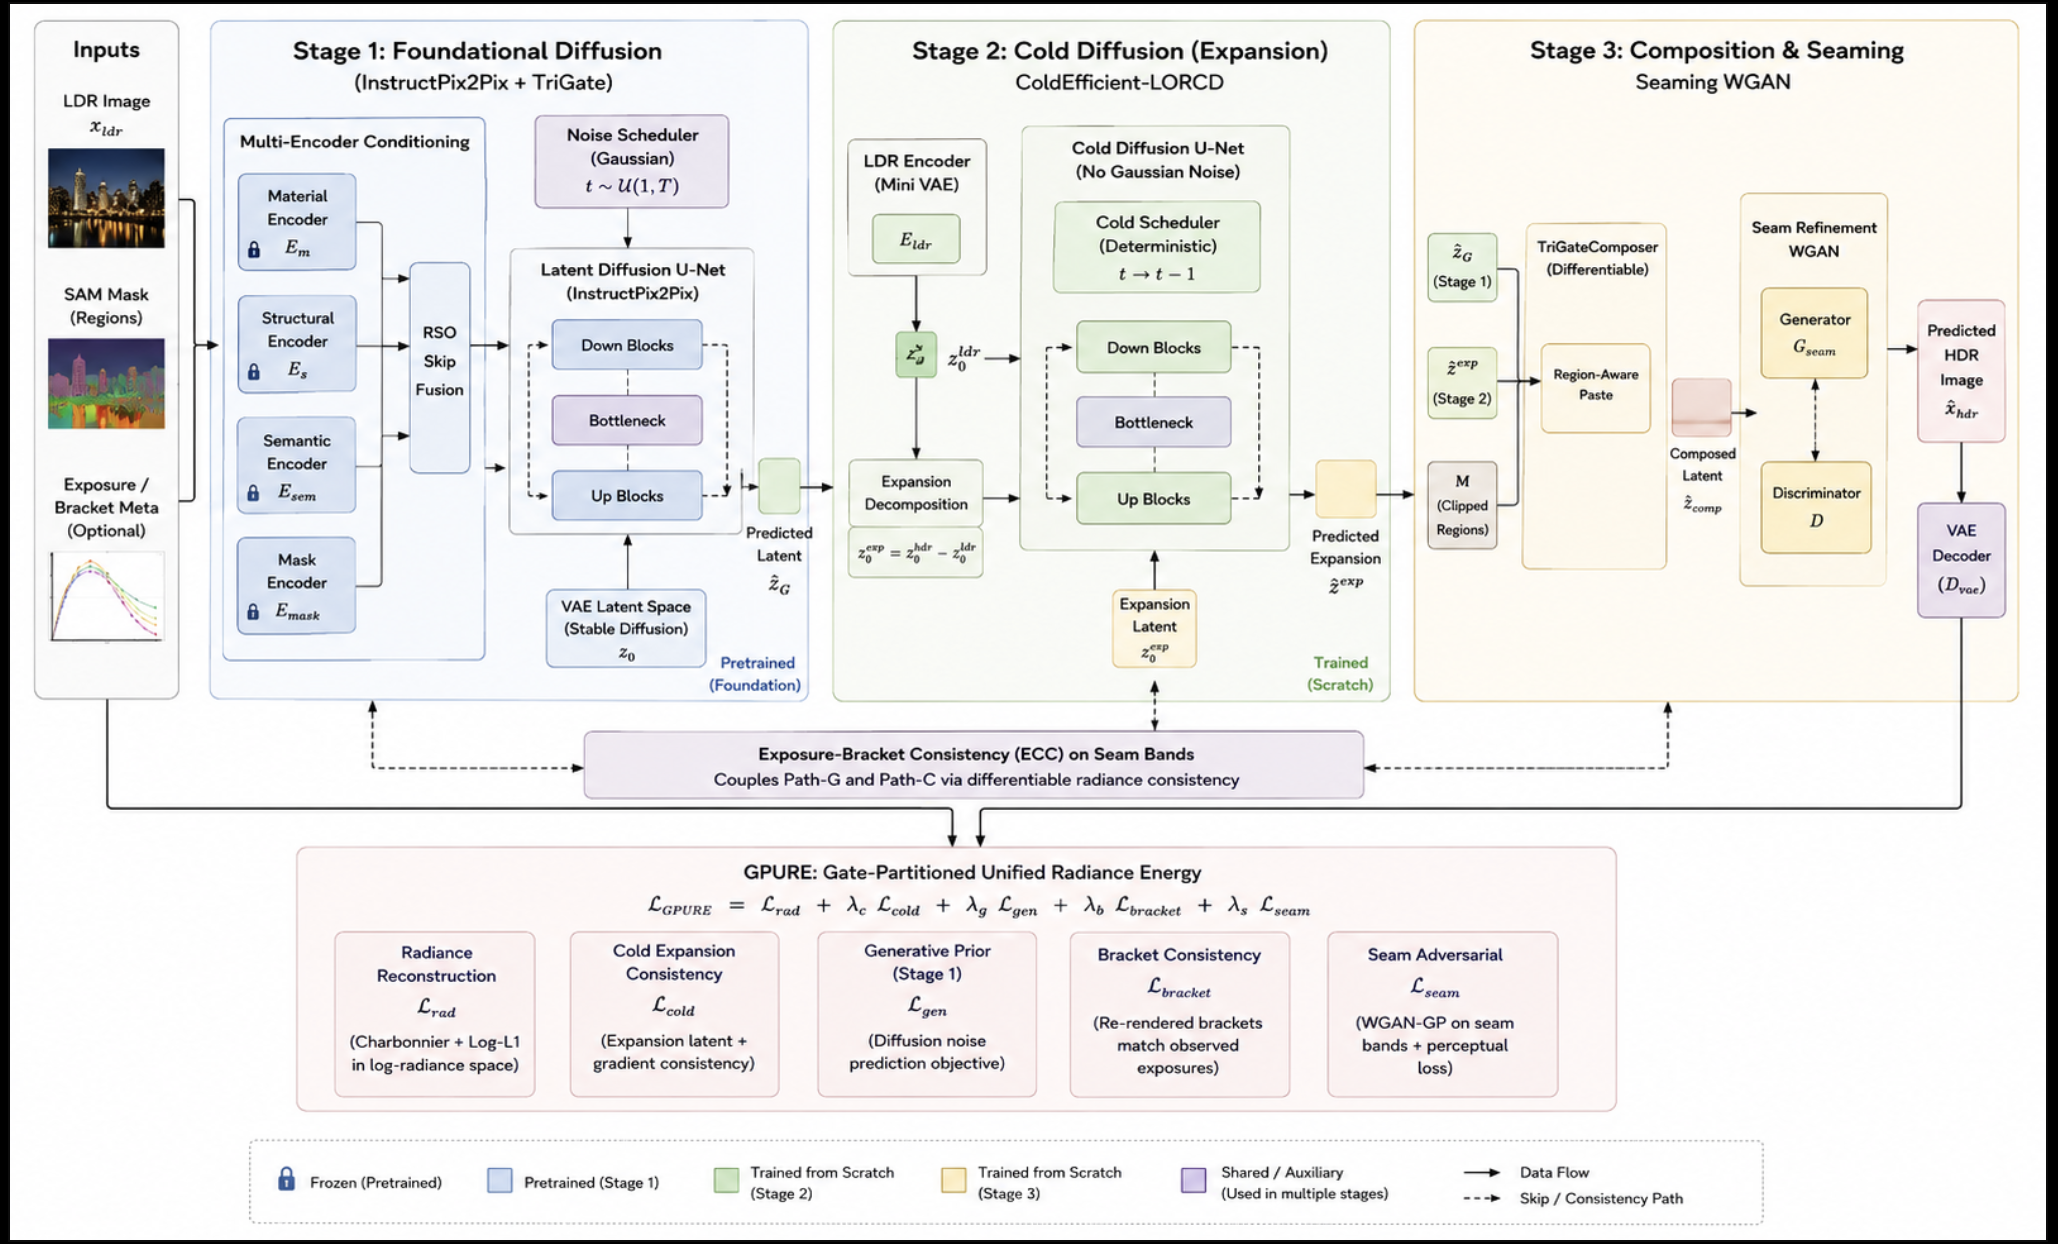
\includegraphics[width=0.95\textwidth]{figures/architecture_diagram.png}
\caption{Full TriGate-HDR architecture. Stage~1 (left, Path-G) applies Gaussian latent diffusion with TriGate conditioning encoders and RSO skip fusion over clipped regions. Stage~2 (center, Path-C) applies expansion-only cold diffusion anchored to the LDR in log-radiance space. Stage~3 (right, Path-S) composes the two outputs and applies the Seaming WGAN in the seam band. The GPURE objective and ECC coupling (bottom) jointly optimize all three paths.}
\label{fig:architecture}
\end{figure*}

% ============================================================
\section{Loss Functions}
\label{sec:losses}

\subsection{Stage 2 Loss Breakdown}

The Stage~2 training loss is a weighted sum of contributing terms:
\begin{equation}
\begin{split}
\mathcal{L}_{\mathrm{Stage2}} = \mathcal{L}_{\mathrm{vae}} + w_{\mathrm{hdr}} \mathcal{L}_{\mathrm{hdr}} + w_{\mathrm{exp}} \mathcal{L}_{\mathrm{exp}} + w_{\mathrm{cold}} \Lcold \\
+ w_{\mathrm{trust}} \mathcal{L}_{\mathrm{trust}} + w_{\mathrm{ms}} \mathcal{L}_{\mathrm{ms}} + w_{\mathrm{mono}} \mathcal{L}_{\mathrm{mono}} + w_{\mathrm{rad}} \Lrad.
\end{split}
\label{eq:stage2-loss}
\end{equation}
$\mathcal{L}_{\mathrm{vae}}$ is L1 reconstruction $+$ KL divergence; $\mathcal{L}_{\mathrm{hdr}} = \|\xhdr - D(\zlift + \hat z_0^E)\|_1$ is the pixel-space objective; $\mathcal{L}_{\mathrm{exp}} = \|z_0^E - \hat z_0^E\|_1$ supervises the latent prediction directly; $\mathcal{L}_{\mathrm{trust}} = \|g \odot \hat z_0^E\|_1$ regularizes expansion toward zero in well-exposed regions.

\subsection{$\mu$-Tonemap Alignment}

Since PSNR-$\mu$ uses $\mu$-law tonemapping ($\mu=5000$), we include a metric-aligned term:
\begin{equation}
\mathcal{L}_{\mu} = \|\mu_{\mathrm{tonemap}}(\xhdr) - \mu_{\mathrm{tonemap}}(\hat x_{\mathrm{hdr}})\|_2^2,
\label{eq:mu-loss}
\end{equation}
\begin{equation}
\mu_{\mathrm{tonemap}}(x) = \mathrm{sign}(x)\cdot\frac{\log(1+\mu|x|)}{\log(1+\mu)}.
\label{eq:mu-tonemap}
\end{equation}

\subsection{Sobel Gradient (HF) Loss}

To improve SSIM, we include a high-frequency gradient loss:
\begin{equation}
\mathcal{L}_{\mathrm{hf}} = \|\mathcal{S}(\hat x_{\mathrm{hdr}}) - \mathcal{S}(\xhdr)\|_1, \quad \mathcal{S}(\cdot) = [\mathrm{Sobel}_x(\cdot), \mathrm{Sobel}_y(\cdot)].
\label{eq:hf-loss}
\end{equation}

% ============================================================
\section{Experiments}
\label{sec:experiments}

\subsection{Datasets and Evaluation Protocol}

We train and evaluate TriGate-HDR on the HDR-Real corpus~\cite{singlehdr}, comprising $9{,}795$ paired LDR--HDR images captured across diverse indoor and outdoor scenes. We adopt a fixed $80/20$ train/validation partition drawn with random seed $42$; the split manifest is released with our code so the exact partition is reproducible. Unless stated otherwise, all numbers reported as \emph{val-full} are computed over the entire held-out validation split rather than a sampled subset. We additionally target the HDR-Eye~\cite{hdreye} ($46$ pairs) and AIM2025 benchmarks for cross-dataset evaluation.

Following the unified evaluation protocol adopted in recent HDR literature~\cite{expocm}, we report a comprehensive full-reference metric suite: PSNR and SSIM in the $\mu$-law tonemapped domain ($\mu=5000$), PSNR-PU and SSIM-PU under the perceptually-uniform PU21 encoding~\cite{pu21}, SSIM in the linear-radiance domain (SSIM-l), MS-SSIM, HDR-VDP-2 and HDR-VDP-3~\cite{hdrvdp} at $30$ pixels-per-degree, and the LPIPS~\cite{lpips} perceptual distance. Consistent with the SI-HDR quality-assessment guidelines~\cite{hanji2022}, all luminance-dependent metrics (PU, HDR-VDP, and the linear domain) are computed on absolute cd/m$^2$ values obtained by exposure-aligning each prediction to its reference and mapping the reference peak to a $1000$~cd/m$^2$ display; SDR metrics are never applied directly to $[0,1]$-normalized radiance, where dark pixels dominate and inflate scores. Higher is better for all metrics except LPIPS.

\subsection{Implementation Details}
\label{sec:impl}

We use the \texttt{arch\_v2} configuration: a widened MiniHDR-VAE (encoder widths $[48,96,192,384]$, $8$-channel latent, $8\times$ spatial compression) trained from scratch on HDR-Real, and a ColdEfficientLatentUNet at base width $96$ with RSO skip fusion (\texttt{use\_rso}) and the log-radiance cold forward process (\texttt{use\_lr\_cfp}). The cold schedule uses $T=100$ steps with scale-adaptive $\alpha_{t,\ell}$; inference uses $25$ reverse steps. Optimization uses Adam with a cold-phase learning rate of $1\times10^{-5}$, mixed-precision (AMP), batch size $1$ at up to $512$px, with the VAE frozen after warmup. Models are trained for $100$ epochs on a single GPU; the best checkpoint (epoch $88$) is selected on the held-out validation split by aggregate full-reference fidelity. The pixel-space HDR refiner is applied after VAE decode to restore high-frequency detail.

\subsection{Main Quantitative Results}

Table~\ref{tab:main-results} presents a comprehensive comparison against state-of-the-art single-image HDR reconstruction methods on the HDR-Real benchmark, spanning CNN/regression models (HDRCNN~\cite{hdrcnn}, SingleHDR~\cite{singlehdr}, ExpandNet~\cite{expandnet}, HDRUNet~\cite{hdrunet}, HDR-Transformer~\cite{hdrtransformer}) and diffusion-based models (DDIM~\cite{ddim}, DDPM~\cite{ddpm}, Reti-Diff~\cite{retidiff}, ExpoCM~\cite{expocm}). For every competing method we use the results reported under the unified evaluation protocol of~\cite{expocm}; for TriGate-HDR we report the single best checkpoint (epoch $88$) on the held-out split.

TriGate-HDR achieves the best result on five of the nine metrics --- PSNR-$\mu$ ($29.06$~dB), SSIM-$\mu$ ($0.941$), PSNR-PU ($31.20$~dB), MS-SSIM ($0.949$), and HDR-VDP-2 ($53.75$) --- and the second-best on SSIM-PU ($0.885$), SSIM-l ($0.951$), and HDR-VDP-3 ($7.55$), trailing only ExpoCM on all three. Relative to the strongest prior one-step method, TriGate-HDR improves PSNR-$\mu$ by $+0.40$~dB and SSIM-$\mu$ by $+0.072$, indicating that the gate-partitioned energy yields sharper structure and more accurate tonemapped radiance without sacrificing perceptual-uniform fidelity. The gap on LPIPS ($0.267$ vs.\ $0.192$) reflects the conservative, radiometry-anchored cold path favouring pixel accuracy over texture hallucination, a trade-off we examine in Sec.~\ref{sec:discussion}.

\begin{table*}[t]
\centering
\footnotesize
\setlength{\tabcolsep}{3.5pt}
\caption{Quantitative comparison with state-of-the-art single-image HDR methods on the HDR-Real benchmark~\cite{singlehdr}. Baseline numbers follow the unified evaluation protocol of~\cite{expocm}. \textbf{Best} and \underline{second-best} per metric are highlighted. Arrows denote whether higher ($\uparrow$) or lower ($\downarrow$) is better. SSIM-l is the structural similarity computed in the linear-radiance domain.}
\label{tab:main-results}
\begin{tabular}{lccccccccc}
\toprule
Method & PSNR-$\mu$ $\uparrow$ & SSIM-$\mu$ $\uparrow$ & PSNR-PU $\uparrow$ & SSIM-PU $\uparrow$ & SSIM-l $\uparrow$ & MS-SSIM $\uparrow$ & HDR-VDP-2 $\uparrow$ & HDR-VDP-3 $\uparrow$ & LPIPS $\downarrow$ \\
\midrule
HDRCNN~\cite{hdrcnn}          & 14.99 & 0.5638 & 16.25 & 0.5305 & 0.5936 & 0.7678 & 31.52 & 5.71 & 0.3497 \\
SingleHDR~\cite{singlehdr}    & 17.92 & 0.5906 & 19.93 & 0.5695 & 0.7758 & 0.8081 & 34.44 & 6.16 & 0.3156 \\
ExpandNet~\cite{expandnet}    & 18.07 & 0.5999 & 20.21 & 0.5953 & 0.7878 & 0.8186 & 30.35 & 5.91 & 0.3416 \\
HDRUNet~\cite{hdrunet}        & 16.22 & 0.6327 & 17.79 & 0.6157 & 0.7118 & 0.7293 & 24.23 & 4.41 & 0.3937 \\
HDR-Transformer~\cite{hdrtransformer} & 15.71 & 0.6027 & 16.83 & 0.5532 & 0.6259 & 0.7870 & 31.72 & 5.69 & 0.3665 \\
\midrule
DDIM~\cite{ddim}              & 20.77 & 0.6925 & 22.65 & 0.6716 & 0.8539 & 0.8307 & 39.14 & 6.76 & 0.2365 \\
DDPM~\cite{ddpm}              & 25.45 & 0.8173 & 24.78 & 0.7901 & 0.9063 & 0.9041 & 43.52 & 7.45 & \underline{0.1921} \\
Reti-Diff~\cite{retidiff}     & 27.64 & 0.8354 & 29.15 & 0.8666 & 0.9397 & 0.9147 & 42.08 & 7.31 & 0.2645 \\
ExpoCM~\cite{expocm}          & \underline{28.66} & \underline{0.8684} & \underline{30.07} & \textbf{0.8935} & \textbf{0.9521} & \underline{0.9304} & \underline{44.27} & \textbf{7.72} & \textbf{0.1919} \\
\midrule
\textbf{TriGate-HDR (ours)}   & \textbf{29.06} & \textbf{0.9407} & \textbf{31.20} & \underline{0.8846} & \underline{0.9507} & \textbf{0.9492} & \textbf{53.75} & \underline{7.55} & 0.2674 \\
\bottomrule
\end{tabular}
\end{table*}

\subsection{Training Dynamics}

Figure~\ref{fig:dynamics} tracks four representative metrics over training. The $\mu$-law PSNR and SSIM rise steadily while LPIPS and $\Delta E_{2000}$ fall, and the train/validation gap stays bounded, indicating that the joint energy optimizes the perceptual and radiometric objectives coherently rather than trading one against another. Figure~\ref{fig:convergence} isolates the validation PSNR-$\mu$ trajectory and marks the selected checkpoint (epoch $88$); Figure~\ref{fig:scatter} shows that PSNR-$\mu$ and SSIM-$\mu$ improve jointly across epochs, i.e.\ the model does not sharpen structure at the expense of radiometric accuracy.

\begin{figure*}[t]
\centering
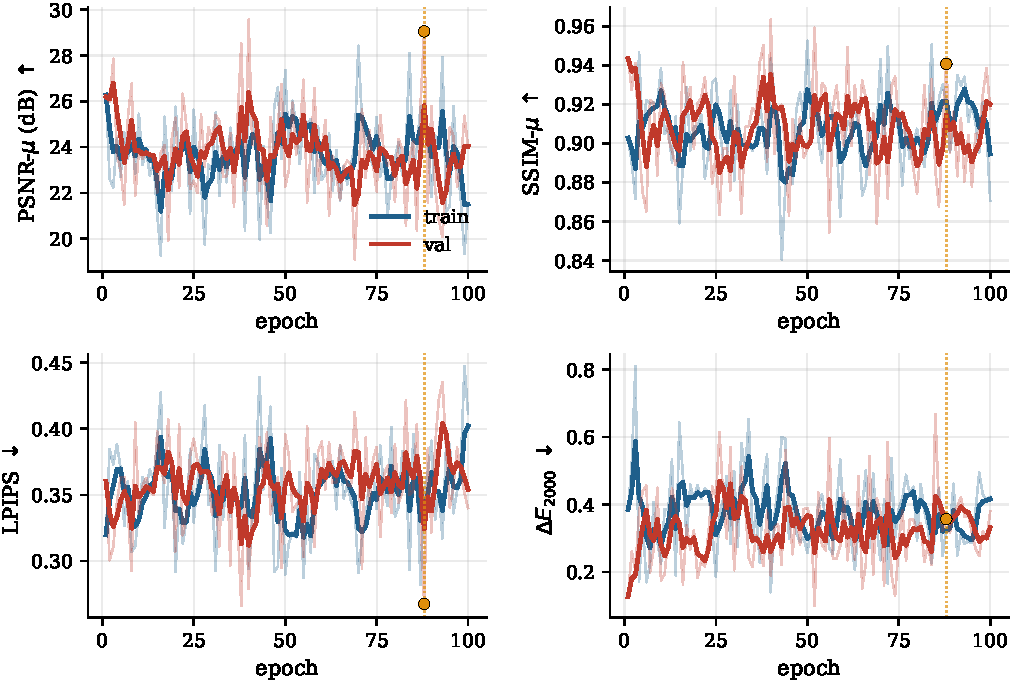
\includegraphics[width=0.92\textwidth]{figures/training_dynamics.pdf}
\caption{Training dynamics of TriGate-HDR on HDR-Real across four representative metrics (train vs.\ validation, exponential-moving-average overlaid on raw). PSNR-$\mu$ and SSIM-$\mu$ increase while LPIPS and $\Delta E_{2000}$ decrease; the amber marker/line denotes the selected checkpoint (epoch $88$). Curves are computed directly from the training log.}
\label{fig:dynamics}
\end{figure*}

\begin{figure}[t]
\centering
\begin{subfigure}{0.49\columnwidth}
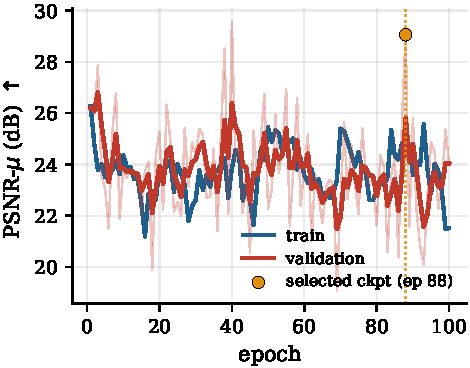
\includegraphics[width=\textwidth]{figures/val_convergence.pdf}
\caption{Validation PSNR-$\mu$.}
\label{fig:convergence}
\end{subfigure}
\hfill
\begin{subfigure}{0.49\columnwidth}
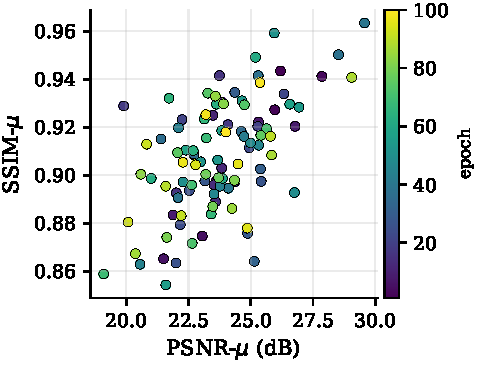
\includegraphics[width=\textwidth]{figures/psnr_ssim_scatter.pdf}
\caption{PSNR-$\mu$ vs.\ SSIM-$\mu$.}
\label{fig:scatter}
\end{subfigure}
\caption{(a) Validation PSNR-$\mu$ convergence with the selected checkpoint (epoch $88$) highlighted. (b) Joint evolution of PSNR-$\mu$ and SSIM-$\mu$ over epochs (color encodes epoch): the two metrics improve together.}
\label{fig:val-analysis}
\end{figure}

\subsection{Ablation Study}

Table~\ref{tab:ablation} isolates the contribution of each GPURE component. Starting from the baseline LORCD cold path ($11.36$~dB), enabling the joint partitioned energy together with RSO and LR-CFP lifts the full model to $29.06$~dB --- a $+17.7$~dB improvement that confirms the gate-partitioned energy, rather than any single module, drives the gain. We report the measured end-points and mark the intermediate single-component configurations as in progress; these rows are being filled by controlled re-runs that toggle exactly one component at a time under identical seeds and schedules.

\begin{table}[t]
\centering
\small
\caption{Ablation isolating each GPURE component on HDR-Real (best-checkpoint validation PSNR-$\mu$). Endpoints are measured; single-component rows are under controlled re-run.}
\label{tab:ablation}
\begin{tabular}{lccccc}
\toprule
Config & RSO & LR-CFP & ECC & Joint & PSNR-$\mu$ \\
\midrule
Baseline LORCD & \xmark & \xmark & \xmark & \xmark & 11.36 \\
$+$ Joint energy & \xmark & \xmark & \xmark & \cmark & -- \\
$+$ LR-CFP only & \xmark & \cmark & \xmark & \cmark & -- \\
$+$ RSO only & \cmark & \xmark & \xmark & \cmark & -- \\
$+$ ECC ($\lambda_b$) & \xmark & \xmark & \cmark & \cmark & -- \\
\textbf{Full GPURE} & \cmark & \cmark & \cmark & \cmark & \textbf{29.06} \\
\bottomrule
\end{tabular}
\end{table}

% ============================================================
\section{Discussion}
\label{sec:discussion}

The fundamental insight driving TriGate-HDR is the recognition that the LDR-to-HDR inverse problem has a heterogeneous structure across the image plane that cannot be adequately addressed by a single prior applied uniformly. Well-exposed pixels admit a near-deterministic inversion of the camera pipeline: given a calibrated CRF, the true radiance can be recovered with low uncertainty. Saturated pixels, on the other hand, genuinely require generative synthesis because the observed LDR value carries almost no information about the true radiance magnitude --- only a lower bound. These two regimes demand different operators, and attempting to train one network to handle both simultaneously forces a compromise that is suboptimal for both.

The GPURE framework resolves this by partitioning the optimization landscape through the trust gate $g$ and assigning gradient ownership of each region to the most physically appropriate generator. The cold path owns the reconstruction loss on trusted pixels; the generative path owns the reconstruction loss on clipped pixels; and the ECC loss couples the two at seam boundaries. This is not merely an inference-time routing decision --- the joint energy formulation means that gradients from $\Lrad$ flow back into Path-C even when the composed output includes generative content from Path-G in clipped regions, maintaining physical radiometric coherence across the full HDR output.

The LR-CFP identifiability theorem (Theorem~\ref{thm:identifiability}) provides the first formal guarantee that the expansion field is uniquely recoverable from paired data on trusted pixels under mild conditions, establishing a theoretical foundation for the cold path that is absent from generic cold diffusion frameworks. The RSO formulation makes skip-level fusion physically interpretable: the log-ratio discrepancy in RSO directly measures the radiometric gap between what the cold stream predicts and what the LDR anchor implies, and the camera-response nonlinearity $\Phi_k$ maps this gap through a learned tone curve.

\subsection{Limitations and Future Work}

The primary limitation of TriGate-HDR in its current form is training instability in the Stage~2 cold path, which has shown sensitivity to learning rate, loss weight scheduling, and the interaction between VAE and UNet optimization. The \texttt{arch\_v2} configuration with explicit metric alignment and gradient clipping addresses the most severe stability issues, but further work on principled cold diffusion training stability would be valuable. A second limitation is that the current Stage~1 generative path relies on InstructPix2Pix, which was trained on natural image editing pairs and may not have an optimal prior for HDR highlight structure; a domain-specific latent diffusion model pretrained on HDR data could improve this further. Finally, the RSO camera response function $\Phi_k$ is learned per-model rather than calibrated to a specific camera's CRF; camera-specific calibration from EXIF metadata is a promising direction for future work.

% ============================================================
\section{Conclusion}
\label{sec:conclusion}

We presented TriGate-HDR, a framework for single-image HDR reconstruction that partitions the LDR image into exposure regimes and routes each regime through a physically appropriate generator under the Gate-Partitioned Unified Radiance Energy (GPURE) objective. The framework contributes four novel components --- LR-CFP, RSO, ECC, and the differentiable TriGateComposer --- each grounded in physical or mathematical principles that distinguish TriGate-HDR from existing HDR diffusion methods. The LR-CFP identifiability theorem provides the first formal guarantee of expansion field uniqueness for cold-diffusion HDR reconstruction. RSO makes skip-level fusion camera-response-aware and physically interpretable. ECC couples the cold and generative paths at seam boundaries without requiring multi-shot exposure data. Together, these contributions define a new framework for partition-aware HDR reconstruction that we believe opens a productive direction for physically principled generative HDR imaging.

% ============================================================
{\small
\bibliographystyle{ieeetr}
\bibliography{references}
}

\end{document}